
\section{Aula 6.3 - Multiplexação por divisão no tempo I}

Nessa aula é introduzido o importantíssimo conceito de multiplexação e a multiplexação de divisão no tempo o que são frames e time slots
\\\\
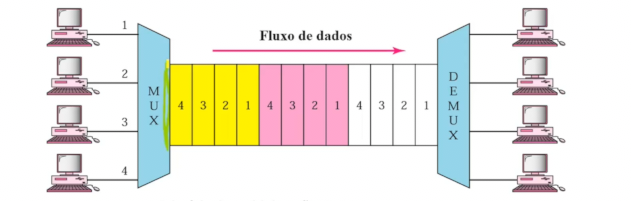
\includegraphics[width=0.6\textwidth]{../assets/muxte.png}

\subsection{O que é multiplexar?}

A idea é que uma interface, no contexto de comunicações geralmente um meio físico como fio, é conectada a múltiplas fontes de sinal e escolhe qual sinal deseja transmitir
baseado em algum critério.


\subsection{Como conceitualmente ocorre a multiplexação de divisão no tempo}

\subsubsection{O que é TDM}
A TDM(time divison multiplexing) ou multiplexação de divisão no tempo é o critério de tempo isto é a banda de transmissão é particionada para alocar diferentes fontes de sinal.
No nosso contexto o sinal vem da entidade tributário que paga para uma companhia telefônica para ter acesso a rede.

\subsubsection{O que são frames e time slots?}

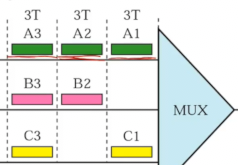
\includegraphics[width=0.4\textwidth]{../assets/tsl.png}
\\\\
Na figura acima fica evidente que há uma certa hierarquia na TDM os frames são blocos de dados com parcelas dos dados produzidos por cada tributário que é enviado num certo período
os time slots são justamente essa parcela de dados previamente mencionada, note que tecnicamente o sistema de comunicação poderia permitir que apenas um tributário usasse a rede por vez
isto é ficar alternando entre tributários por algum critério, mas aí a taxa de envio percebida por um tributário seria abismal essa tradeoff do TDM permite que todos os tributários tenham uma experiência
previsível e justa, visto que a cada, segundo a imagem, 3T s se passam cada tributário enviou parte de seus dados, enquanto que no outro caso seria 3T*(\#tributarios-1) ou seja
linear a complexidade computacional.

\subsection{O bit de sincronização}

Bem para o receptor conseguir decodificar corretamente a menssagem é importante garantir que o pacote recebido, o frame, seja de fato o que se espera e não houve
corrupções no envio para isso é adotado um bit de sincronização que segue um padrão interno que consegue validar a ordem de recebimento de pacotes e garantir a leitura correta
dos bits enviados por cada tributário.




